
\begin{figure*}[ht!]
	\centering
	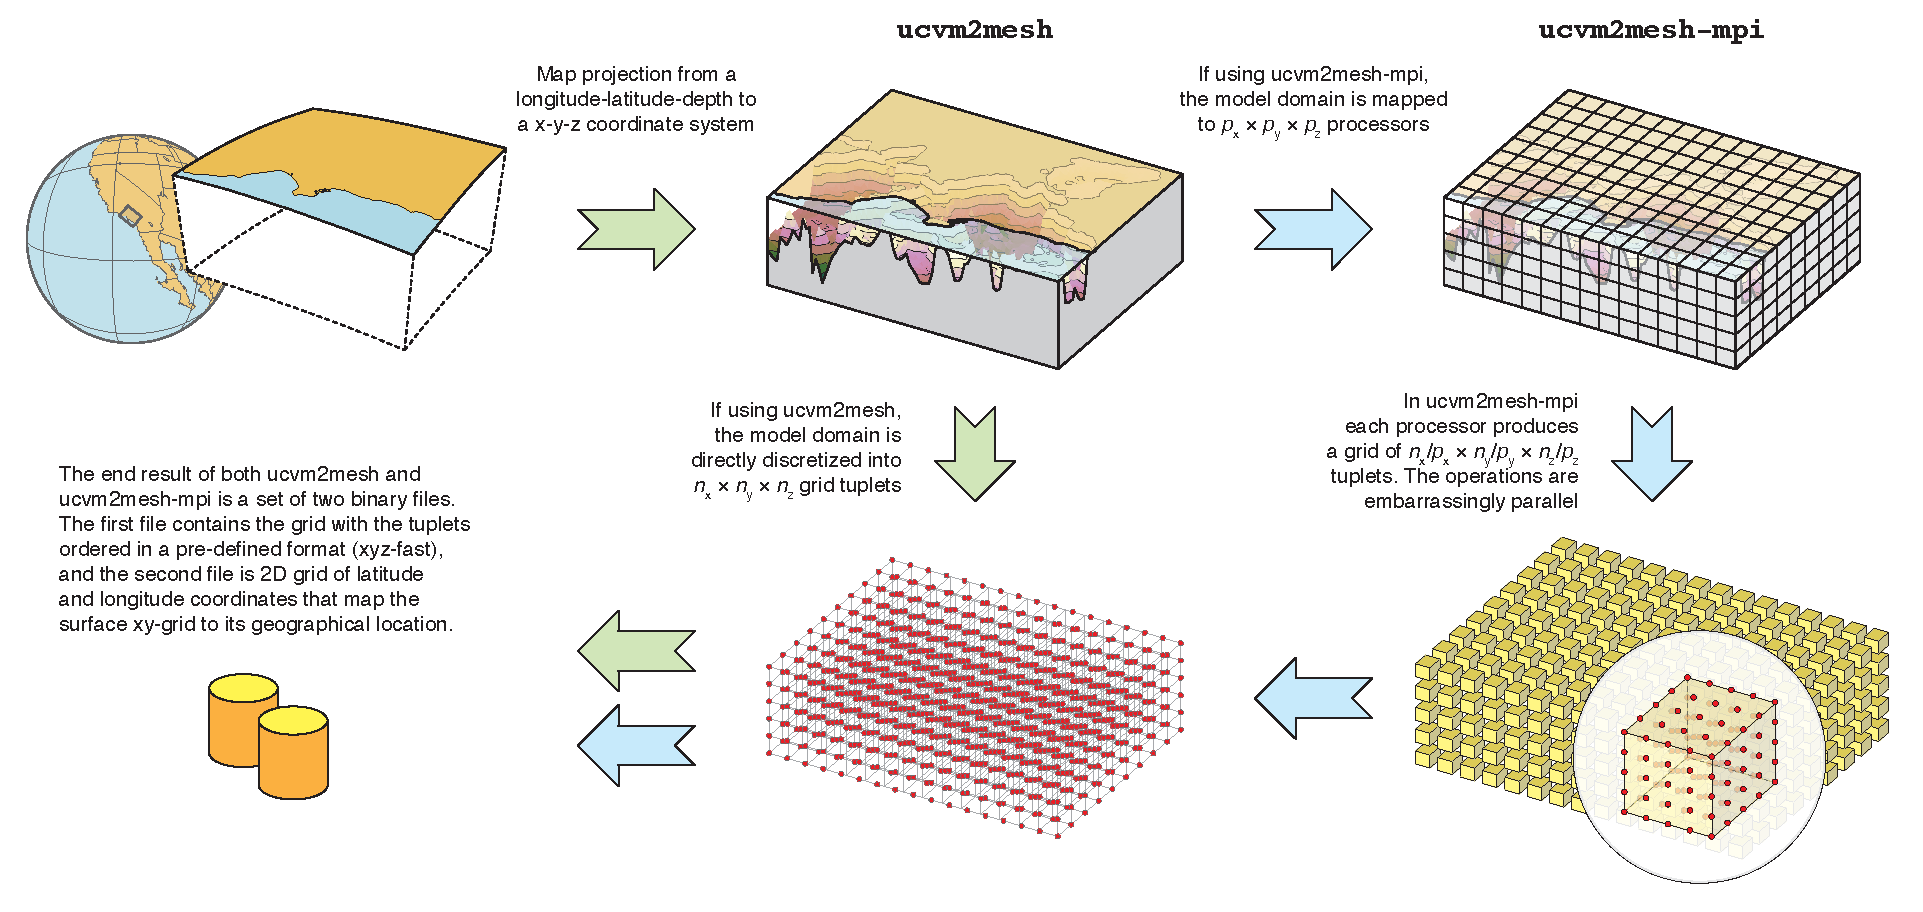
\includegraphics
		[width=\textwidth]
		{figures/pdf/ucvm-to-mesh}
	\caption{Construction of a structured grid with the programs \texttt{ucvm2mesh} (green arrows) and \texttt{ucvm2mesh-mpi} (blue arrows). An important aspect of the gridding process is that the discretized information payload (\vs{}, \vp{}, and $\rho$) is stored at the grid points. That is, the querying and assignment process has a 1-to-1 mapping between the queried point and the grid node of the mesh.}
	\label{fig:meshing}
\end{figure*}
